\documentclass[twoside]{book}

% Packages required by doxygen
\usepackage{fixltx2e}
\usepackage{calc}
\usepackage{doxygen}
\usepackage[export]{adjustbox} % also loads graphicx
\usepackage{graphicx}
\usepackage[utf8]{inputenc}
\usepackage{makeidx}
\usepackage{multicol}
\usepackage{multirow}
\PassOptionsToPackage{warn}{textcomp}
\usepackage{textcomp}
\usepackage[nointegrals]{wasysym}
\usepackage[table]{xcolor}

% Font selection
\usepackage[T1]{fontenc}
\usepackage[scaled=.90]{helvet}
\usepackage{courier}
\usepackage{amssymb}
\usepackage{sectsty}
\renewcommand{\familydefault}{\sfdefault}
\allsectionsfont{%
  \fontseries{bc}\selectfont%
  \color{darkgray}%
}
\renewcommand{\DoxyLabelFont}{%
  \fontseries{bc}\selectfont%
  \color{darkgray}%
}
\newcommand{\+}{\discretionary{\mbox{\scriptsize$\hookleftarrow$}}{}{}}

% Page & text layout
\usepackage{geometry}
\geometry{%
  a4paper,%
  top=2.5cm,%
  bottom=2.5cm,%
  left=2.5cm,%
  right=2.5cm%
}
\tolerance=750
\hfuzz=15pt
\hbadness=750
\setlength{\emergencystretch}{15pt}
\setlength{\parindent}{0cm}
\setlength{\parskip}{3ex plus 2ex minus 2ex}
\makeatletter
\renewcommand{\paragraph}{%
  \@startsection{paragraph}{4}{0ex}{-1.0ex}{1.0ex}{%
    \normalfont\normalsize\bfseries\SS@parafont%
  }%
}
\renewcommand{\subparagraph}{%
  \@startsection{subparagraph}{5}{0ex}{-1.0ex}{1.0ex}{%
    \normalfont\normalsize\bfseries\SS@subparafont%
  }%
}
\makeatother

% Headers & footers
\usepackage{fancyhdr}
\pagestyle{fancyplain}
\fancyhead[LE]{\fancyplain{}{\bfseries\thepage}}
\fancyhead[CE]{\fancyplain{}{}}
\fancyhead[RE]{\fancyplain{}{\bfseries\leftmark}}
\fancyhead[LO]{\fancyplain{}{\bfseries\rightmark}}
\fancyhead[CO]{\fancyplain{}{}}
\fancyhead[RO]{\fancyplain{}{\bfseries\thepage}}
\fancyfoot[LE]{\fancyplain{}{}}
\fancyfoot[CE]{\fancyplain{}{}}
\fancyfoot[RE]{\fancyplain{}{\bfseries\scriptsize Generated by Doxygen }}
\fancyfoot[LO]{\fancyplain{}{\bfseries\scriptsize Generated by Doxygen }}
\fancyfoot[CO]{\fancyplain{}{}}
\fancyfoot[RO]{\fancyplain{}{}}
\renewcommand{\footrulewidth}{0.4pt}
\renewcommand{\chaptermark}[1]{%
  \markboth{#1}{}%
}
\renewcommand{\sectionmark}[1]{%
  \markright{\thesection\ #1}%
}

% Indices & bibliography
\usepackage{natbib}
\usepackage[titles]{tocloft}
\setcounter{tocdepth}{3}
\setcounter{secnumdepth}{5}
\makeindex

% Hyperlinks (required, but should be loaded last)
\usepackage{ifpdf}
\ifpdf
  \usepackage[pdftex,pagebackref=true]{hyperref}
\else
  \usepackage[ps2pdf,pagebackref=true]{hyperref}
\fi
\hypersetup{%
  colorlinks=true,%
  linkcolor=blue,%
  citecolor=blue,%
  unicode%
}

% Custom commands
\newcommand{\clearemptydoublepage}{%
  \newpage{\pagestyle{empty}\cleardoublepage}%
}

\usepackage{caption}
\captionsetup{labelsep=space,justification=centering,font={bf},singlelinecheck=off,skip=4pt,position=top}

%===== C O N T E N T S =====

\begin{document}

% Titlepage & ToC
\hypersetup{pageanchor=false,
             bookmarksnumbered=true,
             pdfencoding=unicode
            }
\pagenumbering{roman}
\begin{titlepage}
\vspace*{7cm}
\begin{center}%
{\Large cell\+Uview \\[1ex]\large 1.\+0.\+0 }\\
\vspace*{1cm}
{\large Generated by Doxygen 1.8.11}\\
\end{center}
\end{titlepage}
\clearemptydoublepage
\tableofcontents
\clearemptydoublepage
\pagenumbering{arabic}
\hypersetup{pageanchor=true}

%--- Begin generated contents ---
\chapter{Hierarchical Index}
\section{Class Hierarchy}
This inheritance list is sorted roughly, but not completely, alphabetically\+:\begin{DoxyCompactList}
\item \contentsline{section}{cell\+Uview\+Welcome}{\pageref{classcell_uview_welcome}}{}
\item \contentsline{section}{frame}{\pageref{classframe}}{}
\item \contentsline{section}{Gallery}{\pageref{class_gallery}}{}
\item \contentsline{section}{image\+Processor}{\pageref{classimage_processor}}{}
\begin{DoxyCompactList}
\item \contentsline{section}{Camera}{\pageref{class_camera}}{}
\item \contentsline{section}{contrast\+Enhancement}{\pageref{classcontrast_enhancement}}{}
\item \contentsline{section}{dilation}{\pageref{classdilation}}{}
\item \contentsline{section}{edge\+Detection}{\pageref{classedge_detection}}{}
\item \contentsline{section}{erosion}{\pageref{classerosion}}{}
\item \contentsline{section}{flat\+Field\+Correct}{\pageref{classflat_field_correct}}{}
\item \contentsline{section}{gray\+Scale}{\pageref{classgray_scale}}{}
\item \contentsline{section}{Gui}{\pageref{class_gui}}{}
\end{DoxyCompactList}
\item Q\+Widget\begin{DoxyCompactList}
\item \contentsline{section}{Gui}{\pageref{class_gui}}{}
\end{DoxyCompactList}
\end{DoxyCompactList}

\chapter{Class Index}
\doxysection{Class List}
Here are the classes, structs, unions and interfaces with brief descriptions\+:\begin{DoxyCompactList}
\item\contentsline{section}{\mbox{\hyperlink{class_camera}{Camera}} }{\pageref{class_camera}}{}
\item\contentsline{section}{\mbox{\hyperlink{classcell_uview_welcome}{cell\+Uview\+Welcome}} }{\pageref{classcell_uview_welcome}}{}
\item\contentsline{section}{\mbox{\hyperlink{classcontrast_enhancement}{contrast\+Enhancement}} }{\pageref{classcontrast_enhancement}}{}
\item\contentsline{section}{\mbox{\hyperlink{classdilation}{dilation}} }{\pageref{classdilation}}{}
\item\contentsline{section}{\mbox{\hyperlink{classedge_detection}{edge\+Detection}} }{\pageref{classedge_detection}}{}
\item\contentsline{section}{\mbox{\hyperlink{classerosion}{erosion}} }{\pageref{classerosion}}{}
\item\contentsline{section}{\mbox{\hyperlink{classflat_field_correct}{flat\+Field\+Correct}} }{\pageref{classflat_field_correct}}{}
\item\contentsline{section}{\mbox{\hyperlink{classframe}{frame}} }{\pageref{classframe}}{}
\item\contentsline{section}{\mbox{\hyperlink{class_gallery}{Gallery}} }{\pageref{class_gallery}}{}
\item\contentsline{section}{\mbox{\hyperlink{classgray_scale}{gray\+Scale}} }{\pageref{classgray_scale}}{}
\item\contentsline{section}{\mbox{\hyperlink{class_gui}{Gui}} }{\pageref{class_gui}}{}
\item\contentsline{section}{\mbox{\hyperlink{classimage_processor}{image\+Processor}} }{\pageref{classimage_processor}}{}
\end{DoxyCompactList}

\chapter{Class Documentation}
\hypertarget{class_camera}{}\doxysection{Camera Class Reference}
\label{class_camera}\index{Camera@{Camera}}
Inheritance diagram for Camera\+:\begin{figure}[H]
\begin{center}
\leavevmode
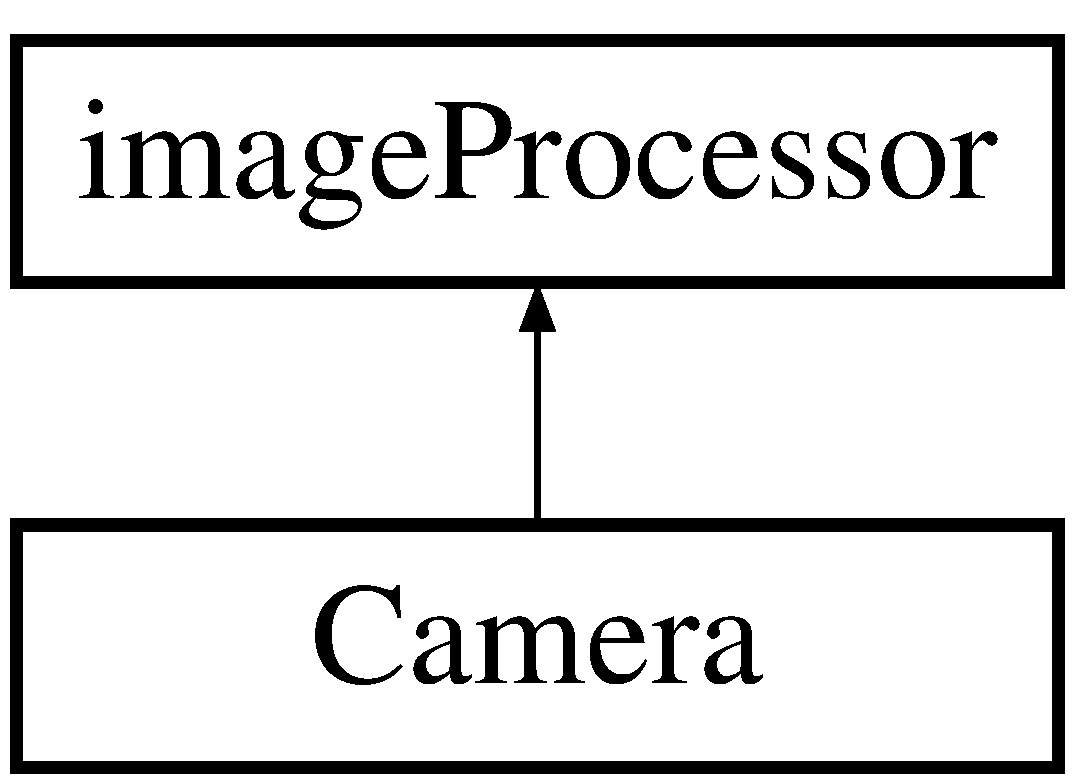
\includegraphics[height=2.000000cm]{class_camera}
\end{center}
\end{figure}
\doxysubsection*{Public Member Functions}
\begin{DoxyCompactItemize}
\item 
\mbox{\Hypertarget{class_camera_a3cd0cd6f746715260f64551803379883}\label{class_camera_a3cd0cd6f746715260f64551803379883}} 
void {\bfseries start} (int device\+ID=0, int api\+ID=0)
\item 
\mbox{\Hypertarget{class_camera_ae6c6aeaf70ad261f3c188c50e8701b0b}\label{class_camera_ae6c6aeaf70ad261f3c188c50e8701b0b}} 
void {\bfseries stop} ()
\item 
\mbox{\Hypertarget{class_camera_a83396433ca6457173dc1844152715de2}\label{class_camera_a83396433ca6457173dc1844152715de2}} 
bool {\bfseries get\+Is\+On} ()
\item 
\mbox{\Hypertarget{class_camera_a974535be48b49903ad17d3fd456c6b1c}\label{class_camera_a974535be48b49903ad17d3fd456c6b1c}} 
void {\bfseries capture\+Metadata} ()
\item 
\mbox{\Hypertarget{class_camera_aff550113223c8cb6f9c3dcead5dce65b}\label{class_camera_aff550113223c8cb6f9c3dcead5dce65b}} 
void {\bfseries set\+Exposure} (int)
\item 
std\+::string \mbox{\hyperlink{class_camera_a9bc9cf6296523cdb0c6e1b7c7b8de1e0}{get\+Param\+Label}} ()
\item 
void \mbox{\hyperlink{class_camera_ae6c8345e9a3b08dd698058db6d858ca2}{update\+Settings}} (std\+::map$<$ std\+::string, std\+::string $>$)
\item 
void \mbox{\hyperlink{class_camera_ab49cc3479fe3a8aee5964a560af918ea}{receive\+Frame}} (\mbox{\hyperlink{classframe}{frame}} new\+Frame)
\end{DoxyCompactItemize}
\doxysubsection*{Additional Inherited Members}


\doxysubsection{Member Function Documentation}
\mbox{\Hypertarget{class_camera_a9bc9cf6296523cdb0c6e1b7c7b8de1e0}\label{class_camera_a9bc9cf6296523cdb0c6e1b7c7b8de1e0}} 
\index{Camera@{Camera}!getParamLabel@{getParamLabel}}
\index{getParamLabel@{getParamLabel}!Camera@{Camera}}
\doxysubsubsection{\texorpdfstring{getParamLabel()}{getParamLabel()}}
{\footnotesize\ttfamily std\+::string Camera\+::get\+Param\+Label (\begin{DoxyParamCaption}{ }\end{DoxyParamCaption})\hspace{0.3cm}{\ttfamily [inline]}, {\ttfamily [virtual]}}



Implements \mbox{\hyperlink{classimage_processor}{image\+Processor}}.

\mbox{\Hypertarget{class_camera_ab49cc3479fe3a8aee5964a560af918ea}\label{class_camera_ab49cc3479fe3a8aee5964a560af918ea}} 
\index{Camera@{Camera}!receiveFrame@{receiveFrame}}
\index{receiveFrame@{receiveFrame}!Camera@{Camera}}
\doxysubsubsection{\texorpdfstring{receiveFrame()}{receiveFrame()}}
{\footnotesize\ttfamily void Camera\+::receive\+Frame (\begin{DoxyParamCaption}\item[{\mbox{\hyperlink{classframe}{frame}}}]{new\+Frame }\end{DoxyParamCaption})\hspace{0.3cm}{\ttfamily [inline]}, {\ttfamily [virtual]}}



Implements \mbox{\hyperlink{classimage_processor}{image\+Processor}}.

\mbox{\Hypertarget{class_camera_ae6c8345e9a3b08dd698058db6d858ca2}\label{class_camera_ae6c8345e9a3b08dd698058db6d858ca2}} 
\index{Camera@{Camera}!updateSettings@{updateSettings}}
\index{updateSettings@{updateSettings}!Camera@{Camera}}
\doxysubsubsection{\texorpdfstring{updateSettings()}{updateSettings()}}
{\footnotesize\ttfamily void Camera\+::update\+Settings (\begin{DoxyParamCaption}\item[{std\+::map$<$ std\+::string, std\+::string $>$}]{metadata }\end{DoxyParamCaption})\hspace{0.3cm}{\ttfamily [virtual]}}



Implements \mbox{\hyperlink{classimage_processor}{image\+Processor}}.



The documentation for this class was generated from the following files\+:\begin{DoxyCompactItemize}
\item 
src/camera.\+h\item 
src/camera.\+cpp\end{DoxyCompactItemize}

\hypertarget{classcell_uview_welcome}{}\doxysection{cell\+Uview\+Welcome Class Reference}
\label{classcell_uview_welcome}\index{cellUviewWelcome@{cellUviewWelcome}}


{\ttfamily \#include $<$cell\+Uview\+Welcome.\+h$>$}

\doxysubsection*{Static Public Member Functions}
\begin{DoxyCompactItemize}
\item 
\mbox{\Hypertarget{classcell_uview_welcome_af2444371dd0d638e07efdcb41eba54aa}\label{classcell_uview_welcome_af2444371dd0d638e07efdcb41eba54aa}} 
static void {\bfseries welcome\+Message} ()
\end{DoxyCompactItemize}


\doxysubsection{Detailed Description}
Prints welcome message ASCII art on application start. 

The documentation for this class was generated from the following file\+:\begin{DoxyCompactItemize}
\item 
src/cell\+Uview\+Welcome.\+h\end{DoxyCompactItemize}

\hypertarget{classcontrast_enhancement}{}\section{contrast\+Enhancement Class Reference}
\label{classcontrast_enhancement}\index{contrast\+Enhancement@{contrast\+Enhancement}}
Inheritance diagram for contrast\+Enhancement\+:\begin{figure}[H]
\begin{center}
\leavevmode
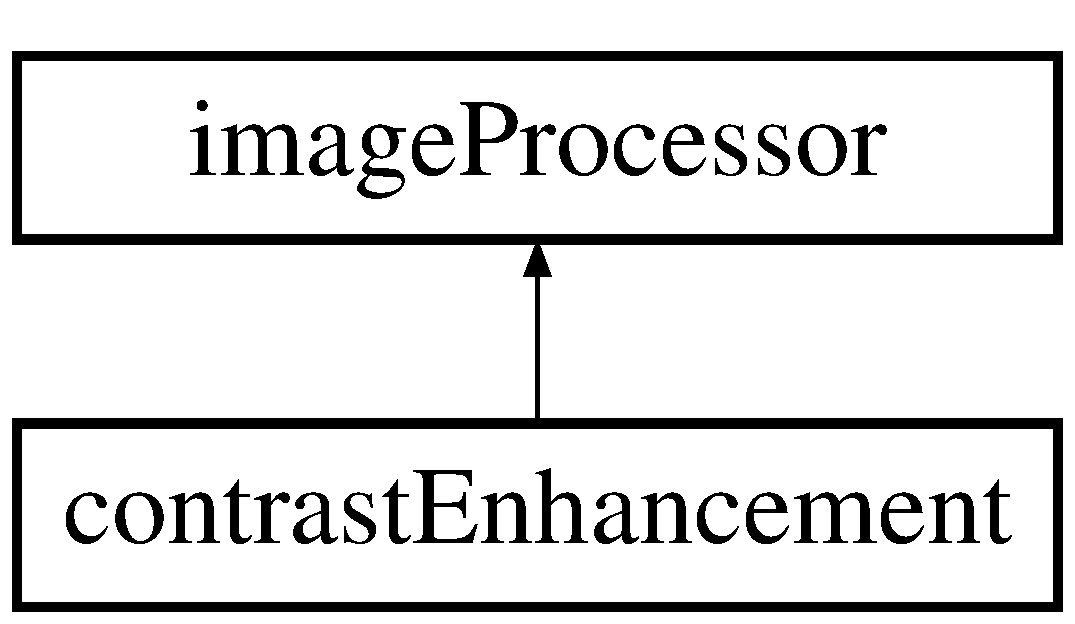
\includegraphics[height=2.000000cm]{classcontrast_enhancement}
\end{center}
\end{figure}
\subsection*{Public Member Functions}
\begin{DoxyCompactItemize}
\item 
void {\bfseries receive\+Frame} (\hyperlink{classframe}{frame} new\+Frame)\hypertarget{classcontrast_enhancement_a2b1c35061a4e24e29f757284ad94327f}{}\label{classcontrast_enhancement_a2b1c35061a4e24e29f757284ad94327f}

\item 
void {\bfseries update\+Threshold} (int value)\hypertarget{classcontrast_enhancement_aa98d801afd8448167834b19eb582db57}{}\label{classcontrast_enhancement_aa98d801afd8448167834b19eb582db57}

\item 
void {\bfseries update\+Settings} (std\+::map$<$ std\+::string, std\+::string $>$)\hypertarget{classcontrast_enhancement_abddfdb4dfb9d762b3a8da187688d2002}{}\label{classcontrast_enhancement_abddfdb4dfb9d762b3a8da187688d2002}

\item 
std\+::string {\bfseries get\+Param\+Label} ()\hypertarget{classcontrast_enhancement_a08c202cd0a1d9dbd7974b6273f0f6ade}{}\label{classcontrast_enhancement_a08c202cd0a1d9dbd7974b6273f0f6ade}

\end{DoxyCompactItemize}
\subsection*{Public Attributes}
\begin{DoxyCompactItemize}
\item 
float {\bfseries threshold} = 0\hypertarget{classcontrast_enhancement_a83f21a927926197fde712d00cf37368d}{}\label{classcontrast_enhancement_a83f21a927926197fde712d00cf37368d}

\item 
float {\bfseries slider\+Threshold} = 10\hypertarget{classcontrast_enhancement_a32768f79d77cd5803078fc5ce97a9230}{}\label{classcontrast_enhancement_a32768f79d77cd5803078fc5ce97a9230}

\end{DoxyCompactItemize}
\subsection*{Additional Inherited Members}


The documentation for this class was generated from the following files\+:\begin{DoxyCompactItemize}
\item 
src/contrast\+Enhancement.\+h\item 
src/contrast\+Enhancement.\+cpp\end{DoxyCompactItemize}

\hypertarget{classdilation}{}\doxysection{dilation Class Reference}
\label{classdilation}\index{dilation@{dilation}}
Inheritance diagram for dilation\+:\begin{figure}[H]
\begin{center}
\leavevmode
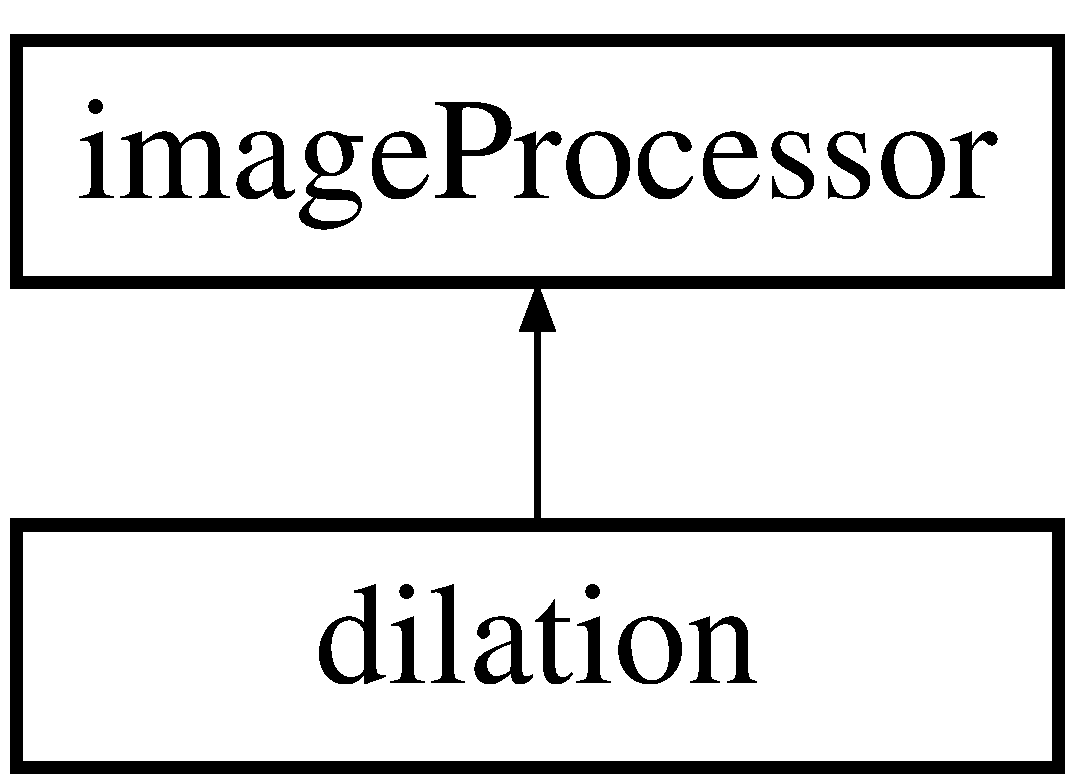
\includegraphics[height=2.000000cm]{classdilation}
\end{center}
\end{figure}
\doxysubsection*{Public Member Functions}
\begin{DoxyCompactItemize}
\item 
void \mbox{\hyperlink{classdilation_ad2edf7b45ead513737cce8ba2190ea38}{receive\+Frame}} (\mbox{\hyperlink{classframe}{frame}} new\+Frame)
\item 
std\+::string \mbox{\hyperlink{classdilation_aac678c6a5fd8a4bcd6e5fd82a4ba9769}{get\+Param\+Label}} ()
\item 
void \mbox{\hyperlink{classdilation_a0c243de870bb878a20c43673e082b953}{update\+Settings}} (std\+::map$<$ std\+::string, std\+::string $>$)
\end{DoxyCompactItemize}
\doxysubsection*{Additional Inherited Members}


\doxysubsection{Member Function Documentation}
\mbox{\Hypertarget{classdilation_aac678c6a5fd8a4bcd6e5fd82a4ba9769}\label{classdilation_aac678c6a5fd8a4bcd6e5fd82a4ba9769}} 
\index{dilation@{dilation}!getParamLabel@{getParamLabel}}
\index{getParamLabel@{getParamLabel}!dilation@{dilation}}
\doxysubsubsection{\texorpdfstring{getParamLabel()}{getParamLabel()}}
{\footnotesize\ttfamily std\+::string dilation\+::get\+Param\+Label (\begin{DoxyParamCaption}{ }\end{DoxyParamCaption})\hspace{0.3cm}{\ttfamily [inline]}, {\ttfamily [virtual]}}



Implements \mbox{\hyperlink{classimage_processor}{image\+Processor}}.

\mbox{\Hypertarget{classdilation_ad2edf7b45ead513737cce8ba2190ea38}\label{classdilation_ad2edf7b45ead513737cce8ba2190ea38}} 
\index{dilation@{dilation}!receiveFrame@{receiveFrame}}
\index{receiveFrame@{receiveFrame}!dilation@{dilation}}
\doxysubsubsection{\texorpdfstring{receiveFrame()}{receiveFrame()}}
{\footnotesize\ttfamily void dilation\+::receive\+Frame (\begin{DoxyParamCaption}\item[{\mbox{\hyperlink{classframe}{frame}}}]{new\+Frame }\end{DoxyParamCaption})\hspace{0.3cm}{\ttfamily [virtual]}}



Implements \mbox{\hyperlink{classimage_processor}{image\+Processor}}.

\mbox{\Hypertarget{classdilation_a0c243de870bb878a20c43673e082b953}\label{classdilation_a0c243de870bb878a20c43673e082b953}} 
\index{dilation@{dilation}!updateSettings@{updateSettings}}
\index{updateSettings@{updateSettings}!dilation@{dilation}}
\doxysubsubsection{\texorpdfstring{updateSettings()}{updateSettings()}}
{\footnotesize\ttfamily void dilation\+::update\+Settings (\begin{DoxyParamCaption}\item[{std\+::map$<$ std\+::string, std\+::string $>$}]{metadata }\end{DoxyParamCaption})\hspace{0.3cm}{\ttfamily [virtual]}}



Implements \mbox{\hyperlink{classimage_processor}{image\+Processor}}.



The documentation for this class was generated from the following files\+:\begin{DoxyCompactItemize}
\item 
/github/workspace/src/dilation.\+h\item 
/github/workspace/src/dilation.\+cpp\end{DoxyCompactItemize}

\hypertarget{classedge_detection}{}\doxysection{edge\+Detection Class Reference}
\label{classedge_detection}\index{edgeDetection@{edgeDetection}}
Inheritance diagram for edge\+Detection\+:\begin{figure}[H]
\begin{center}
\leavevmode
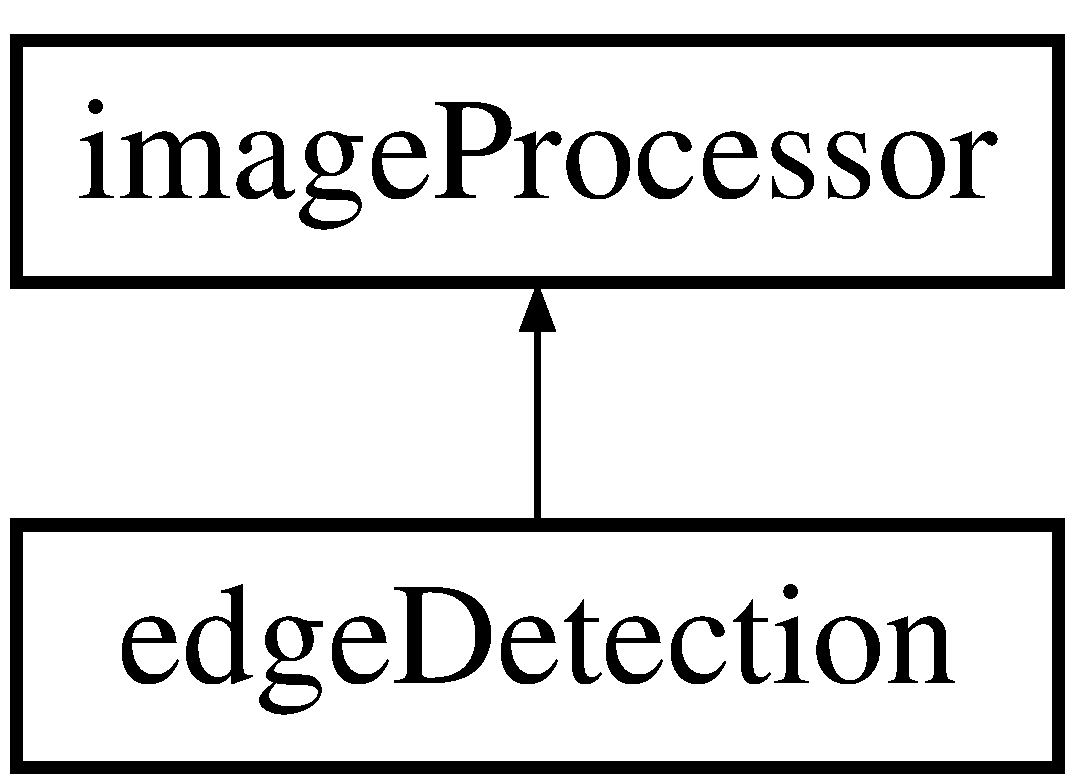
\includegraphics[height=2.000000cm]{classedge_detection}
\end{center}
\end{figure}
\doxysubsection*{Public Member Functions}
\begin{DoxyCompactItemize}
\item 
void \mbox{\hyperlink{classedge_detection_a67bf1c232cd856b735fe5d786cbe30e7}{receive\+Frame}} (\mbox{\hyperlink{classframe}{frame}} new\+Frame)
\item 
\mbox{\Hypertarget{classedge_detection_a4902490150a6371e8ed2c0e99e0e64f5}\label{classedge_detection_a4902490150a6371e8ed2c0e99e0e64f5}} 
void {\bfseries update\+Threshold} (int value)
\item 
void \mbox{\hyperlink{classedge_detection_ad4b2e5b1a4aa3a29c5255f8ab66885d8}{update\+Settings}} (std\+::map$<$ std\+::string, std\+::string $>$)
\item 
std\+::string \mbox{\hyperlink{classedge_detection_af479eae661c2bd12f3bee621a97e15b9}{get\+Param\+Label}} ()
\end{DoxyCompactItemize}
\doxysubsubsection*{Public Member Functions inherited from \mbox{\hyperlink{classimage_processor}{image\+Processor}}}
\begin{DoxyCompactItemize}
\item 
\mbox{\Hypertarget{classimage_processor_a9bf1827b19fcf2d032efd493151c3b5b}\label{classimage_processor_a9bf1827b19fcf2d032efd493151c3b5b}} 
virtual void {\bfseries receive\+Frame} (\mbox{\hyperlink{classframe}{frame}} new\+Frame)=0
\item 
\mbox{\Hypertarget{classimage_processor_af0e1b504003b23c4797acb105faa4aa3}\label{classimage_processor_af0e1b504003b23c4797acb105faa4aa3}} 
virtual void {\bfseries update\+Settings} (std\+::map$<$ std\+::string, std\+::string $>$)=0
\item 
\mbox{\Hypertarget{classimage_processor_a51607435507ae4ff7ecb00ed98f08624}\label{classimage_processor_a51607435507ae4ff7ecb00ed98f08624}} 
virtual std\+::string {\bfseries get\+Param\+Label} ()=0
\item 
\mbox{\Hypertarget{classimage_processor_af3c9e1ed9e62fe3f714a2c637951dc0f}\label{classimage_processor_af3c9e1ed9e62fe3f714a2c637951dc0f}} 
void {\bfseries register\+Callback} (\mbox{\hyperlink{classimage_processor}{image\+Processor}} $\ast$cb)
\item 
\mbox{\Hypertarget{classimage_processor_a7570b72f296fce91a86baf55d2ffc06a}\label{classimage_processor_a7570b72f296fce91a86baf55d2ffc06a}} 
bool {\bfseries toggle\+Enable} ()
\item 
\mbox{\Hypertarget{classimage_processor_a00e2d512096a68f1c3a0866cb7e82d8b}\label{classimage_processor_a00e2d512096a68f1c3a0866cb7e82d8b}} 
bool {\bfseries get\+Enabled} ()
\end{DoxyCompactItemize}
\doxysubsection*{Public Attributes}
\begin{DoxyCompactItemize}
\item 
\mbox{\Hypertarget{classedge_detection_a8e46350aaef5e84ac13d95ec935212a9}\label{classedge_detection_a8e46350aaef5e84ac13d95ec935212a9}} 
int {\bfseries threshold} = 0
\item 
\mbox{\Hypertarget{classedge_detection_a49a4d56a565ef4ba732b19814b8ba7ec}\label{classedge_detection_a49a4d56a565ef4ba732b19814b8ba7ec}} 
int {\bfseries slider\+Threshold} = 100
\end{DoxyCompactItemize}
\doxysubsection*{Additional Inherited Members}
\doxysubsubsection*{Protected Attributes inherited from \mbox{\hyperlink{classimage_processor}{image\+Processor}}}
\begin{DoxyCompactItemize}
\item 
\mbox{\Hypertarget{classimage_processor_a801f1161fd1e94909f93f45fd3391592}\label{classimage_processor_a801f1161fd1e94909f93f45fd3391592}} 
\mbox{\hyperlink{classimage_processor}{image\+Processor}} $\ast$ {\bfseries frame\+Cb} = nullptr
\item 
\mbox{\Hypertarget{classimage_processor_a7d225220555118bc37633cfe8740ae0e}\label{classimage_processor_a7d225220555118bc37633cfe8740ae0e}} 
bool {\bfseries enabled} = false
\end{DoxyCompactItemize}


\doxysubsection{Member Function Documentation}
\mbox{\Hypertarget{classedge_detection_af479eae661c2bd12f3bee621a97e15b9}\label{classedge_detection_af479eae661c2bd12f3bee621a97e15b9}} 
\index{edgeDetection@{edgeDetection}!getParamLabel@{getParamLabel}}
\index{getParamLabel@{getParamLabel}!edgeDetection@{edgeDetection}}
\doxysubsubsection{\texorpdfstring{getParamLabel()}{getParamLabel()}}
{\footnotesize\ttfamily std\+::string edge\+Detection\+::get\+Param\+Label (\begin{DoxyParamCaption}{ }\end{DoxyParamCaption})\hspace{0.3cm}{\ttfamily [inline]}, {\ttfamily [virtual]}}



Implements \mbox{\hyperlink{classimage_processor}{image\+Processor}}.

\mbox{\Hypertarget{classedge_detection_a67bf1c232cd856b735fe5d786cbe30e7}\label{classedge_detection_a67bf1c232cd856b735fe5d786cbe30e7}} 
\index{edgeDetection@{edgeDetection}!receiveFrame@{receiveFrame}}
\index{receiveFrame@{receiveFrame}!edgeDetection@{edgeDetection}}
\doxysubsubsection{\texorpdfstring{receiveFrame()}{receiveFrame()}}
{\footnotesize\ttfamily void edge\+Detection\+::receive\+Frame (\begin{DoxyParamCaption}\item[{\mbox{\hyperlink{classframe}{frame}}}]{new\+Frame }\end{DoxyParamCaption})\hspace{0.3cm}{\ttfamily [virtual]}}



Implements \mbox{\hyperlink{classimage_processor}{image\+Processor}}.

\mbox{\Hypertarget{classedge_detection_ad4b2e5b1a4aa3a29c5255f8ab66885d8}\label{classedge_detection_ad4b2e5b1a4aa3a29c5255f8ab66885d8}} 
\index{edgeDetection@{edgeDetection}!updateSettings@{updateSettings}}
\index{updateSettings@{updateSettings}!edgeDetection@{edgeDetection}}
\doxysubsubsection{\texorpdfstring{updateSettings()}{updateSettings()}}
{\footnotesize\ttfamily void edge\+Detection\+::update\+Settings (\begin{DoxyParamCaption}\item[{std\+::map$<$ std\+::string, std\+::string $>$}]{metadata }\end{DoxyParamCaption})\hspace{0.3cm}{\ttfamily [virtual]}}



Implements \mbox{\hyperlink{classimage_processor}{image\+Processor}}.



The documentation for this class was generated from the following files\+:\begin{DoxyCompactItemize}
\item 
src/edge\+Detection.\+h\item 
src/edge\+Detection.\+cpp\end{DoxyCompactItemize}

\hypertarget{classerosion}{}\section{erosion Class Reference}
\label{classerosion}\index{erosion@{erosion}}
Inheritance diagram for erosion\+:\begin{figure}[H]
\begin{center}
\leavevmode
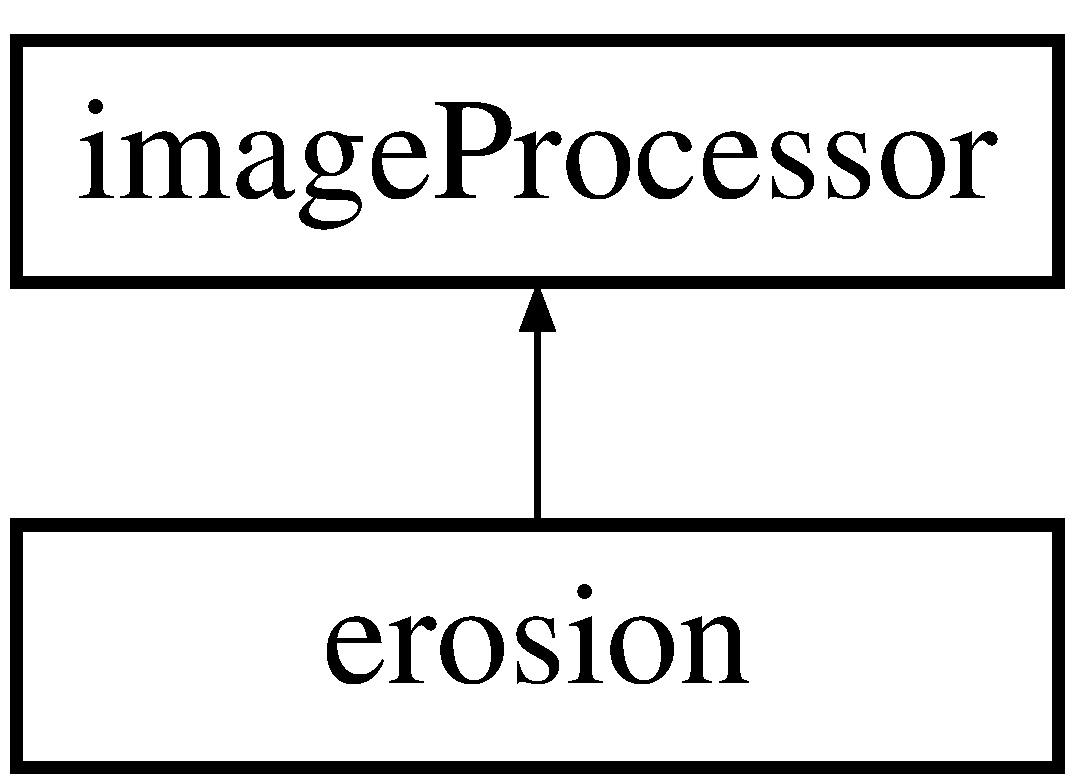
\includegraphics[height=2.000000cm]{classerosion}
\end{center}
\end{figure}
\subsection*{Public Member Functions}
\begin{DoxyCompactItemize}
\item 
void {\bfseries receive\+Frame} (\hyperlink{classframe}{frame} new\+Frame)\hypertarget{classerosion_a40662b6f2b9567d3640bc9d9e6cbd712}{}\label{classerosion_a40662b6f2b9567d3640bc9d9e6cbd712}

\item 
std\+::string {\bfseries get\+Param\+Label} ()\hypertarget{classerosion_a3fa83e64a15e8f6eefede9d3831c3d41}{}\label{classerosion_a3fa83e64a15e8f6eefede9d3831c3d41}

\item 
void {\bfseries update\+Settings} (std\+::map$<$ std\+::string, std\+::string $>$)\hypertarget{classerosion_acb938db0c6a7393a8291baba748e8c50}{}\label{classerosion_acb938db0c6a7393a8291baba748e8c50}

\end{DoxyCompactItemize}
\subsection*{Additional Inherited Members}


The documentation for this class was generated from the following files\+:\begin{DoxyCompactItemize}
\item 
src/erosion.\+h\item 
src/erosion.\+cpp\end{DoxyCompactItemize}

\hypertarget{classflat_field_correct}{}\doxysection{flat\+Field\+Correct Class Reference}
\label{classflat_field_correct}\index{flatFieldCorrect@{flatFieldCorrect}}
Inheritance diagram for flat\+Field\+Correct\+:\begin{figure}[H]
\begin{center}
\leavevmode
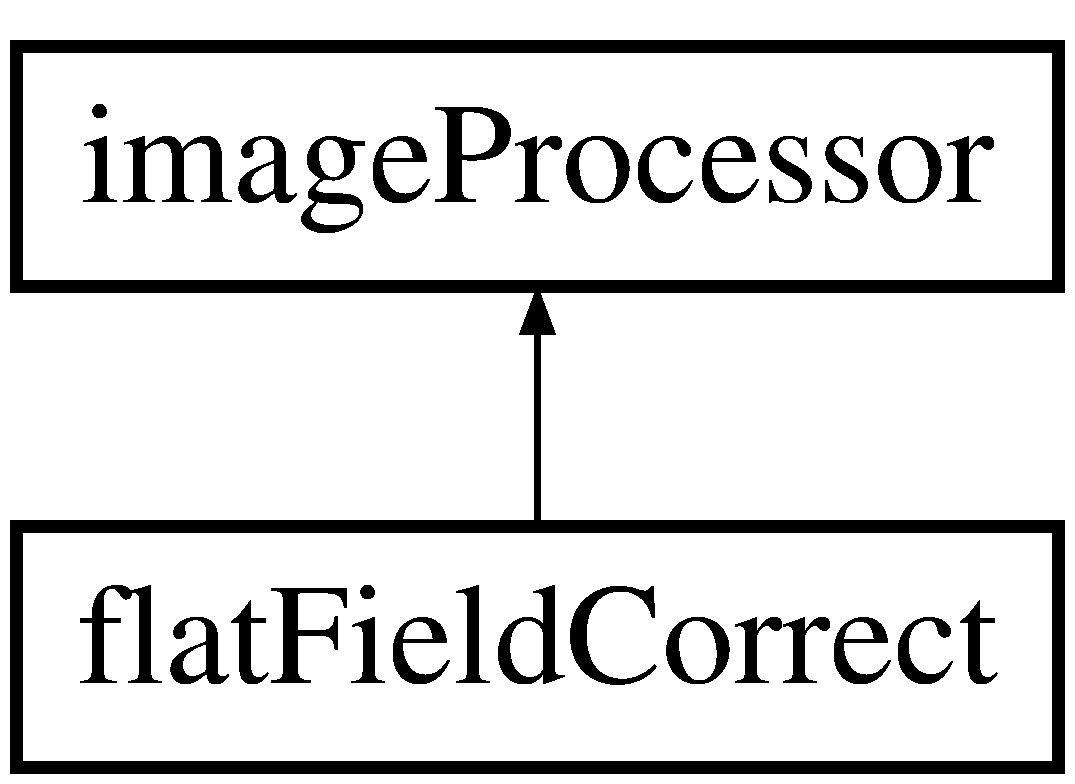
\includegraphics[height=2.000000cm]{classflat_field_correct}
\end{center}
\end{figure}
\doxysubsection*{Public Member Functions}
\begin{DoxyCompactItemize}
\item 
void \mbox{\hyperlink{classflat_field_correct_abb93298ce9ede8bf7dec9ab69acf5555}{receive\+Frame}} (\mbox{\hyperlink{classframe}{frame}} new\+Frame)
\item 
std\+::string \mbox{\hyperlink{classflat_field_correct_a263a8f8f9c0172aa0eed261499510b08}{get\+Param\+Label}} ()
\item 
\mbox{\Hypertarget{classflat_field_correct_a09b0dae1b7251e184b6660655d3b9931}\label{classflat_field_correct_a09b0dae1b7251e184b6660655d3b9931}} 
void {\bfseries set\+Update\+Flag} ()
\item 
void \mbox{\hyperlink{classflat_field_correct_ab6fba6e38ffb4a8f5a9290715afe9b6d}{update\+Settings}} (std\+::map$<$ std\+::string, std\+::string $>$)
\end{DoxyCompactItemize}
\doxysubsection*{Additional Inherited Members}


\doxysubsection{Member Function Documentation}
\mbox{\Hypertarget{classflat_field_correct_a263a8f8f9c0172aa0eed261499510b08}\label{classflat_field_correct_a263a8f8f9c0172aa0eed261499510b08}} 
\index{flatFieldCorrect@{flatFieldCorrect}!getParamLabel@{getParamLabel}}
\index{getParamLabel@{getParamLabel}!flatFieldCorrect@{flatFieldCorrect}}
\doxysubsubsection{\texorpdfstring{getParamLabel()}{getParamLabel()}}
{\footnotesize\ttfamily std\+::string flat\+Field\+Correct\+::get\+Param\+Label (\begin{DoxyParamCaption}{ }\end{DoxyParamCaption})\hspace{0.3cm}{\ttfamily [inline]}, {\ttfamily [virtual]}}



Implements \mbox{\hyperlink{classimage_processor}{image\+Processor}}.

\mbox{\Hypertarget{classflat_field_correct_abb93298ce9ede8bf7dec9ab69acf5555}\label{classflat_field_correct_abb93298ce9ede8bf7dec9ab69acf5555}} 
\index{flatFieldCorrect@{flatFieldCorrect}!receiveFrame@{receiveFrame}}
\index{receiveFrame@{receiveFrame}!flatFieldCorrect@{flatFieldCorrect}}
\doxysubsubsection{\texorpdfstring{receiveFrame()}{receiveFrame()}}
{\footnotesize\ttfamily void flat\+Field\+Correct\+::receive\+Frame (\begin{DoxyParamCaption}\item[{\mbox{\hyperlink{classframe}{frame}}}]{new\+Frame }\end{DoxyParamCaption})\hspace{0.3cm}{\ttfamily [virtual]}}



Implements \mbox{\hyperlink{classimage_processor}{image\+Processor}}.

\mbox{\Hypertarget{classflat_field_correct_ab6fba6e38ffb4a8f5a9290715afe9b6d}\label{classflat_field_correct_ab6fba6e38ffb4a8f5a9290715afe9b6d}} 
\index{flatFieldCorrect@{flatFieldCorrect}!updateSettings@{updateSettings}}
\index{updateSettings@{updateSettings}!flatFieldCorrect@{flatFieldCorrect}}
\doxysubsubsection{\texorpdfstring{updateSettings()}{updateSettings()}}
{\footnotesize\ttfamily void flat\+Field\+Correct\+::update\+Settings (\begin{DoxyParamCaption}\item[{std\+::map$<$ std\+::string, std\+::string $>$}]{metadata }\end{DoxyParamCaption})\hspace{0.3cm}{\ttfamily [virtual]}}



Implements \mbox{\hyperlink{classimage_processor}{image\+Processor}}.



The documentation for this class was generated from the following files\+:\begin{DoxyCompactItemize}
\item 
/github/workspace/src/flat\+Field\+Correct.\+h\item 
/github/workspace/src/flat\+Field\+Correct.\+cpp\end{DoxyCompactItemize}

\hypertarget{classframe}{}\doxysection{frame Class Reference}
\label{classframe}\index{frame@{frame}}
\doxysubsection*{Public Member Functions}
\begin{DoxyCompactItemize}
\item 
\mbox{\Hypertarget{classframe_a30973e896689cd48838800f2ffba8b73}\label{classframe_a30973e896689cd48838800f2ffba8b73}} 
{\bfseries frame} (cv\+::\+Mat mat\+In)
\item 
\mbox{\Hypertarget{classframe_a7f497befd5e8e84ad7e3f67e7b1ce0d5}\label{classframe_a7f497befd5e8e84ad7e3f67e7b1ce0d5}} 
void {\bfseries copy\+From} (\mbox{\hyperlink{classframe}{frame}} $\ast$copy\+From)
\item 
\mbox{\Hypertarget{classframe_a5da1dc6366e266943d87c050f84b1422}\label{classframe_a5da1dc6366e266943d87c050f84b1422}} 
void {\bfseries set\+Parameter} (std\+::string, std\+::string)
\item 
\mbox{\Hypertarget{classframe_abfce006d754b16c702a001f2efd27b1e}\label{classframe_abfce006d754b16c702a001f2efd27b1e}} 
std\+::string {\bfseries encode\+Metadata} ()
\item 
\mbox{\Hypertarget{classframe_af9c18f99fb0ec5174a320c7bd2601b83}\label{classframe_af9c18f99fb0ec5174a320c7bd2601b83}} 
std\+::string {\bfseries get\+Param} (std\+::string)
\item 
\mbox{\Hypertarget{classframe_ab47afb1047012eee24fa2e175c52cde1}\label{classframe_ab47afb1047012eee24fa2e175c52cde1}} 
{\bfseries frame} (\mbox{\hyperlink{classframe}{frame}} const \&)=default
\item 
\mbox{\Hypertarget{classframe_aea4d8c6ae44c207aa6e7130c2abe8e85}\label{classframe_aea4d8c6ae44c207aa6e7130c2abe8e85}} 
int {\bfseries get\+Param\+Size} ()
\end{DoxyCompactItemize}
\doxysubsection*{Public Attributes}
\begin{DoxyCompactItemize}
\item 
\mbox{\Hypertarget{classframe_a718c495452424ccef0090ef136702f02}\label{classframe_a718c495452424ccef0090ef136702f02}} 
cv\+::\+Mat {\bfseries image}
\item 
\mbox{\Hypertarget{classframe_ad7e4a6ba334e987c71f908a2fbbff76c}\label{classframe_ad7e4a6ba334e987c71f908a2fbbff76c}} 
bool {\bfseries do\+Meta} = false
\end{DoxyCompactItemize}


The documentation for this class was generated from the following files\+:\begin{DoxyCompactItemize}
\item 
/github/workspace/src/frame.\+h\item 
/github/workspace/src/frame.\+cpp\end{DoxyCompactItemize}

\hypertarget{class_gallery}{}\doxysection{Gallery Class Reference}
\label{class_gallery}\index{Gallery@{Gallery}}
\doxysubsection*{Public Member Functions}
\begin{DoxyCompactItemize}
\item 
\mbox{\Hypertarget{class_gallery_a110e83aebbb1fc4ec52704df5886be43}\label{class_gallery_a110e83aebbb1fc4ec52704df5886be43}} 
void {\bfseries capture\+Frame} (\mbox{\hyperlink{classframe}{frame}})
\item 
\mbox{\Hypertarget{class_gallery_a5b4879daecb8808cfaf3f8f99c76d348}\label{class_gallery_a5b4879daecb8808cfaf3f8f99c76d348}} 
void {\bfseries update\+Img\+Name} (std\+::string)
\item 
\mbox{\Hypertarget{class_gallery_a2893fa1b10fe346ac865cf8da0d5f08d}\label{class_gallery_a2893fa1b10fe346ac865cf8da0d5f08d}} 
void {\bfseries update\+Index} ()
\item 
\mbox{\Hypertarget{class_gallery_a2f615f26aa87600361856273d2e129b2}\label{class_gallery_a2f615f26aa87600361856273d2e129b2}} 
std\+::map$<$ std\+::string, std\+::string $>$ {\bfseries get\+Metadata} (std\+::string=\char`\"{}\char`\"{})
\item 
\mbox{\Hypertarget{class_gallery_a219722e7c6db614fad9eb055d2d79036}\label{class_gallery_a219722e7c6db614fad9eb055d2d79036}} 
std\+::string {\bfseries get\+Pathname} ()
\item 
\mbox{\Hypertarget{class_gallery_a5c5b3fc09eb83462d9be010a758de18e}\label{class_gallery_a5c5b3fc09eb83462d9be010a758de18e}} 
std\+::string {\bfseries get\+Capture\+Fname} ()
\end{DoxyCompactItemize}


The documentation for this class was generated from the following files\+:\begin{DoxyCompactItemize}
\item 
src/gallery.\+h\item 
src/gallery.\+cpp\end{DoxyCompactItemize}

\hypertarget{classgray_scale}{}\section{gray\+Scale Class Reference}
\label{classgray_scale}\index{gray\+Scale@{gray\+Scale}}
Inheritance diagram for gray\+Scale\+:\begin{figure}[H]
\begin{center}
\leavevmode
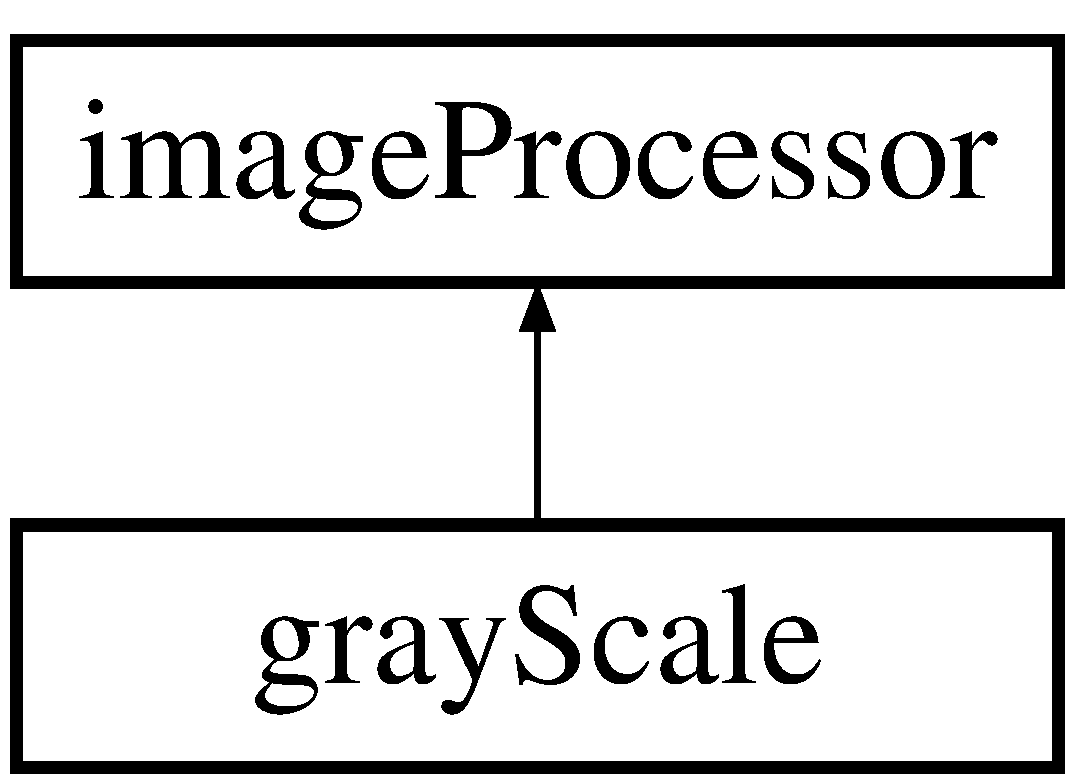
\includegraphics[height=2.000000cm]{classgray_scale}
\end{center}
\end{figure}
\subsection*{Public Member Functions}
\begin{DoxyCompactItemize}
\item 
void {\bfseries receive\+Frame} (\hyperlink{classframe}{frame})\hypertarget{classgray_scale_a2c81c1f679fd56fd705ba0dde71415cd}{}\label{classgray_scale_a2c81c1f679fd56fd705ba0dde71415cd}

\item 
std\+::string {\bfseries get\+Param\+Label} ()\hypertarget{classgray_scale_a55a475e399534ec4e5467c24f0503c2b}{}\label{classgray_scale_a55a475e399534ec4e5467c24f0503c2b}

\item 
void {\bfseries update\+Settings} (std\+::map$<$ std\+::string, std\+::string $>$)\hypertarget{classgray_scale_a509b7f89787c663e8a7312e94d54212d}{}\label{classgray_scale_a509b7f89787c663e8a7312e94d54212d}

\end{DoxyCompactItemize}
\subsection*{Additional Inherited Members}


The documentation for this class was generated from the following files\+:\begin{DoxyCompactItemize}
\item 
src/gray\+Scale.\+h\item 
src/gray\+Scale.\+cpp\end{DoxyCompactItemize}

\hypertarget{class_gui}{}\section{Gui Class Reference}
\label{class_gui}\index{Gui@{Gui}}


{\ttfamily \#include $<$gui.\+h$>$}

Inheritance diagram for Gui\+:\begin{figure}[H]
\begin{center}
\leavevmode
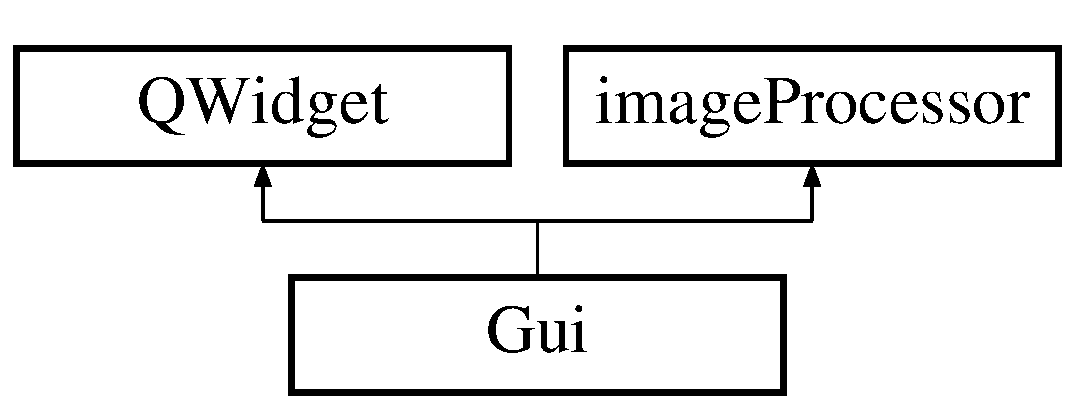
\includegraphics[height=2.000000cm]{class_gui}
\end{center}
\end{figure}
\subsection*{Public Member Functions}
\begin{DoxyCompactItemize}
\item 
void \hyperlink{class_gui_a2f058a424b6584d1907b1f45422da4f6}{receive\+Frame} (\hyperlink{classframe}{frame} new\+Frame)
\item 
\hyperlink{class_gui_a0787d4633eeebebc31ec40ad2b441c25}{Gui} (Q\+Main\+Window $\ast$, Ui\+\_\+\+G\+UI $\ast$, \hyperlink{class_gallery}{Gallery} $\ast$, std\+::vector$<$ \hyperlink{classimage_processor}{image\+Processor} $\ast$ $>$ \&)
\item 
void \hyperlink{class_gui_ac76a8210e18720a6bd248c0f1425a738}{Set\+Visible} (bool visible)
\end{DoxyCompactItemize}
\subsection*{Additional Inherited Members}


\subsection{Detailed Description}
A class which handles G\+UI connections and functionality. 

\subsection{Constructor \& Destructor Documentation}
\index{Gui@{Gui}!Gui@{Gui}}
\index{Gui@{Gui}!Gui@{Gui}}
\subsubsection[{\texorpdfstring{Gui(\+Q\+Main\+Window $\ast$, Ui\+\_\+\+G\+U\+I $\ast$, Gallery $\ast$, std\+::vector$<$ image\+Processor $\ast$ $>$ \&)}{Gui(QMainWindow *, Ui_GUI *, Gallery *, std::vector< imageProcessor * > &)}}]{\setlength{\rightskip}{0pt plus 5cm}Gui\+::\+Gui (
\begin{DoxyParamCaption}
\item[{Q\+Main\+Window $\ast$}]{win, }
\item[{Ui\+\_\+\+G\+UI $\ast$}]{ui\+\_\+win, }
\item[{{\bf Gallery} $\ast$}]{gallery\+In, }
\item[{std\+::vector$<$ {\bf image\+Processor} $\ast$ $>$ \&}]{blocks\+In}
\end{DoxyParamCaption}
)}\hypertarget{class_gui_a0787d4633eeebebc31ec40ad2b441c25}{}\label{class_gui_a0787d4633eeebebc31ec40ad2b441c25}
Constructor to initialise the G\+UI and set connections 
\begin{DoxyParams}{Parameters}
{\em win} & points to Q\+Main\+Window \\
\hline
{\em ui\+\_\+win} & points to Ui\+\_\+\+G\+UI \\
\hline
{\em gallery\+In} & points to \hyperlink{class_gallery}{Gallery} instance \\
\hline
{\em blocks\+In} & is a std\+::vector of the image processing blocks \\
\hline
\end{DoxyParams}


\subsection{Member Function Documentation}
\index{Gui@{Gui}!receive\+Frame@{receive\+Frame}}
\index{receive\+Frame@{receive\+Frame}!Gui@{Gui}}
\subsubsection[{\texorpdfstring{receive\+Frame(frame new\+Frame)}{receiveFrame(frame newFrame)}}]{\setlength{\rightskip}{0pt plus 5cm}void Gui\+::receive\+Frame (
\begin{DoxyParamCaption}
\item[{{\bf frame}}]{new\+Frame}
\end{DoxyParamCaption}
)\hspace{0.3cm}{\ttfamily [virtual]}}\hypertarget{class_gui_a2f058a424b6584d1907b1f45422da4f6}{}\label{class_gui_a2f058a424b6584d1907b1f45422da4f6}
Function to recieve callbacks frames from image processor blocks 
\begin{DoxyParams}{Parameters}
{\em new\+Frame} & frame structure from processing block via callback interface \\
\hline
\end{DoxyParams}


Implements \hyperlink{classimage_processor}{image\+Processor}.

\index{Gui@{Gui}!Set\+Visible@{Set\+Visible}}
\index{Set\+Visible@{Set\+Visible}!Gui@{Gui}}
\subsubsection[{\texorpdfstring{Set\+Visible(bool visible)}{SetVisible(bool visible)}}]{\setlength{\rightskip}{0pt plus 5cm}void Gui\+::\+Set\+Visible (
\begin{DoxyParamCaption}
\item[{bool}]{visible}
\end{DoxyParamCaption}
)}\hypertarget{class_gui_ac76a8210e18720a6bd248c0f1425a738}{}\label{class_gui_ac76a8210e18720a6bd248c0f1425a738}
Sets UI visibility 
\begin{DoxyParams}{Parameters}
{\em visible} & true to make visible \\
\hline
\end{DoxyParams}


The documentation for this class was generated from the following files\+:\begin{DoxyCompactItemize}
\item 
src/gui.\+h\item 
src/gui.\+cpp\end{DoxyCompactItemize}

\hypertarget{classimage_processor}{}\doxysection{image\+Processor Class Reference}
\label{classimage_processor}\index{imageProcessor@{imageProcessor}}
Inheritance diagram for image\+Processor\+:\begin{figure}[H]
\begin{center}
\leavevmode
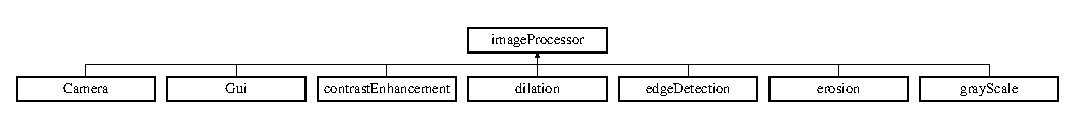
\includegraphics[height=1.134752cm]{classimage_processor}
\end{center}
\end{figure}
\doxysubsection*{Public Member Functions}
\begin{DoxyCompactItemize}
\item 
\mbox{\Hypertarget{classimage_processor_a9bf1827b19fcf2d032efd493151c3b5b}\label{classimage_processor_a9bf1827b19fcf2d032efd493151c3b5b}} 
virtual void {\bfseries receive\+Frame} (\mbox{\hyperlink{classframe}{frame}} new\+Frame)=0
\item 
\mbox{\Hypertarget{classimage_processor_af0e1b504003b23c4797acb105faa4aa3}\label{classimage_processor_af0e1b504003b23c4797acb105faa4aa3}} 
virtual void {\bfseries update\+Settings} (std\+::map$<$ std\+::string, std\+::string $>$)=0
\item 
\mbox{\Hypertarget{classimage_processor_a51607435507ae4ff7ecb00ed98f08624}\label{classimage_processor_a51607435507ae4ff7ecb00ed98f08624}} 
virtual std\+::string {\bfseries get\+Param\+Label} ()=0
\item 
\mbox{\Hypertarget{classimage_processor_af3c9e1ed9e62fe3f714a2c637951dc0f}\label{classimage_processor_af3c9e1ed9e62fe3f714a2c637951dc0f}} 
void {\bfseries register\+Callback} (\mbox{\hyperlink{classimage_processor}{image\+Processor}} $\ast$cb)
\item 
\mbox{\Hypertarget{classimage_processor_a7570b72f296fce91a86baf55d2ffc06a}\label{classimage_processor_a7570b72f296fce91a86baf55d2ffc06a}} 
bool {\bfseries toggle\+Enable} ()
\item 
\mbox{\Hypertarget{classimage_processor_a00e2d512096a68f1c3a0866cb7e82d8b}\label{classimage_processor_a00e2d512096a68f1c3a0866cb7e82d8b}} 
bool {\bfseries get\+Enabled} ()
\end{DoxyCompactItemize}
\doxysubsection*{Protected Attributes}
\begin{DoxyCompactItemize}
\item 
\mbox{\Hypertarget{classimage_processor_a801f1161fd1e94909f93f45fd3391592}\label{classimage_processor_a801f1161fd1e94909f93f45fd3391592}} 
\mbox{\hyperlink{classimage_processor}{image\+Processor}} $\ast$ {\bfseries frame\+Cb} = nullptr
\item 
\mbox{\Hypertarget{classimage_processor_a7d225220555118bc37633cfe8740ae0e}\label{classimage_processor_a7d225220555118bc37633cfe8740ae0e}} 
bool {\bfseries enabled} = false
\end{DoxyCompactItemize}


The documentation for this class was generated from the following file\+:\begin{DoxyCompactItemize}
\item 
src/image\+Processor.\+h\end{DoxyCompactItemize}

%--- End generated contents ---

% Index
\backmatter
\newpage
\phantomsection
\clearemptydoublepage
\addcontentsline{toc}{chapter}{Index}
\printindex

\end{document}
